\section{Modellierung mit Unity}

\subsection{Gelände}
\begin{figure}[h]
\centering
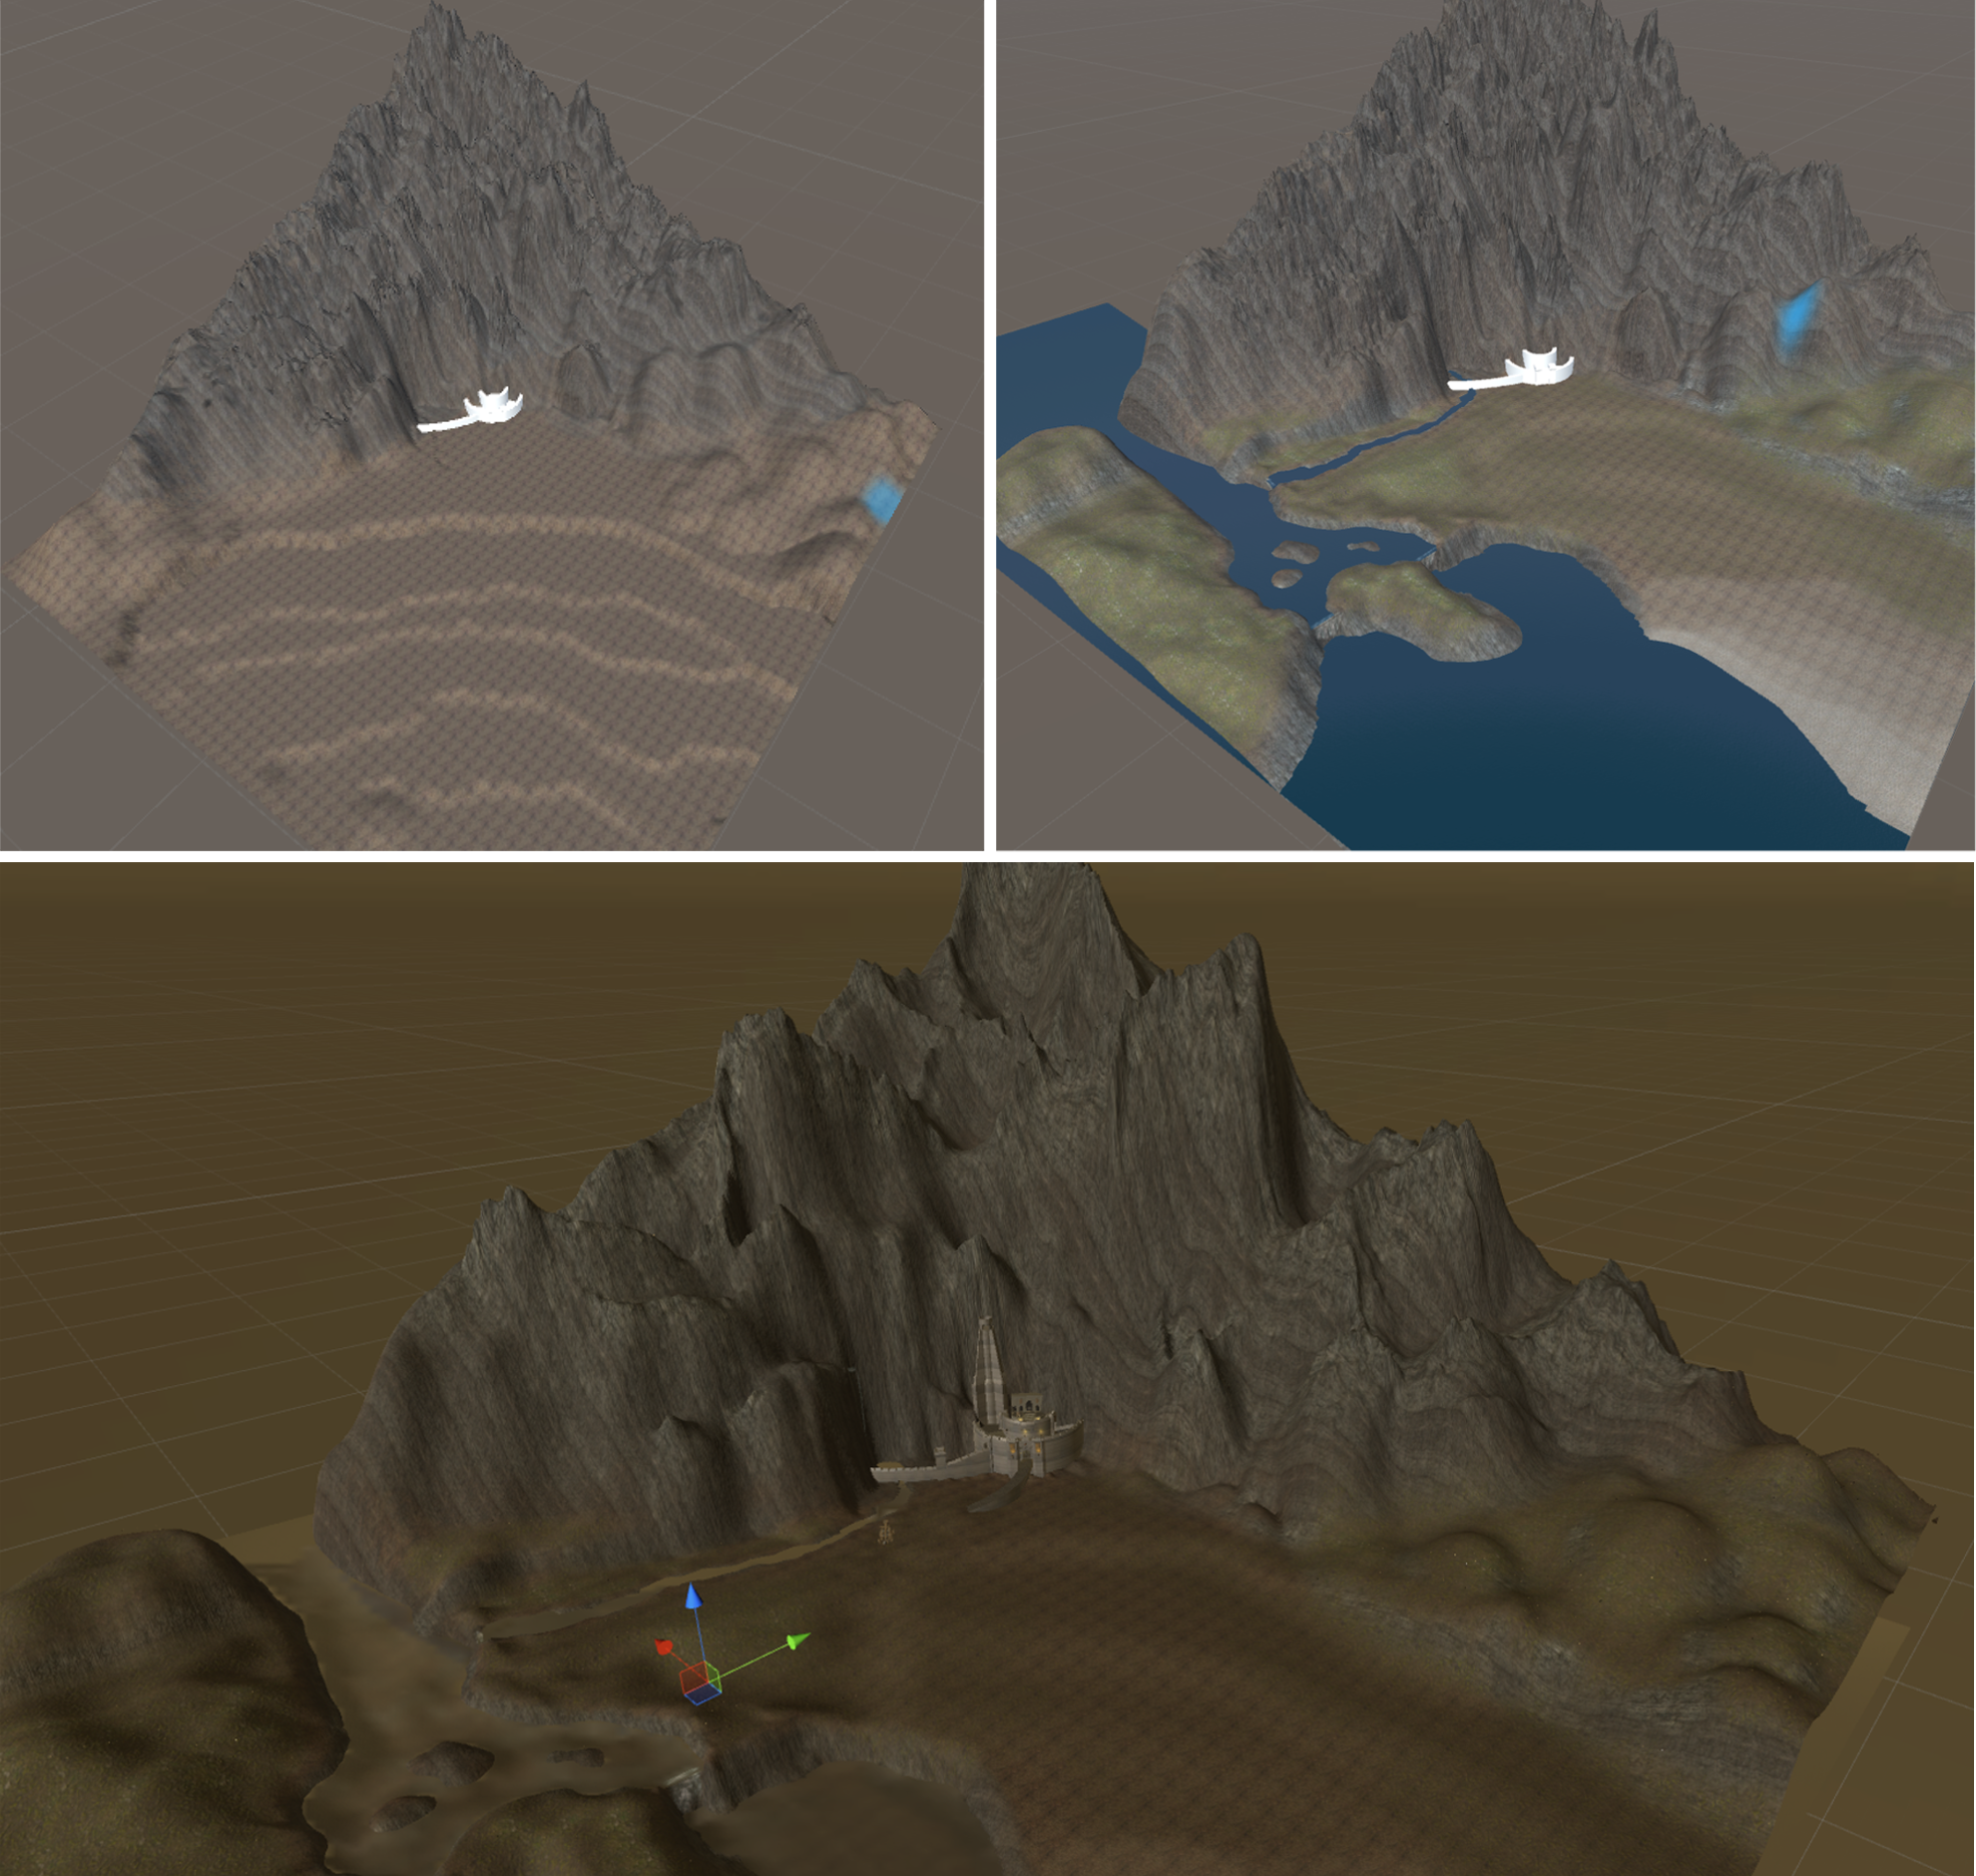
\includegraphics[width=0.95\linewidth]{Abbildungen/Unity/TerrainProgress}
\caption{Entwicklungsschritte des Geländes}
\label{fig:TerrainProgress}
\end{figure}

\begin{wrapfigure}[8]{r}{0.5\textwidth}
	\vspace{-20pt}
	\begin{center}
		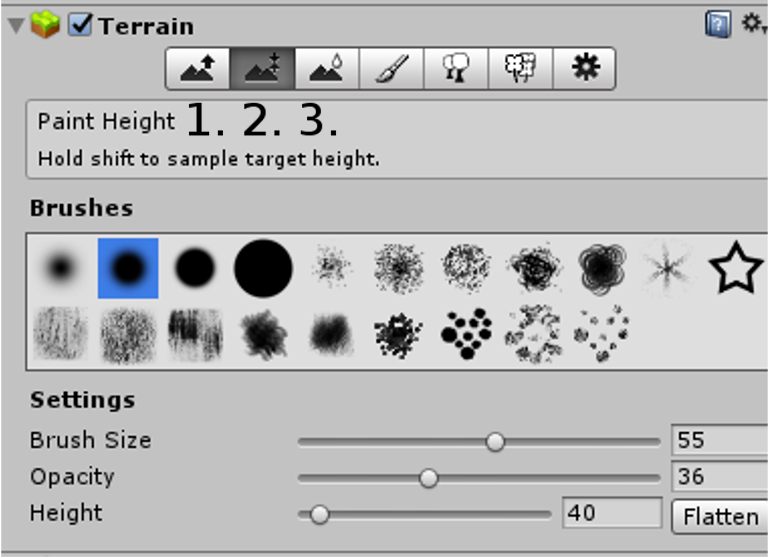
\includegraphics[width=0.45\textwidth]{Abbildungen/Unity/TerrainTool}
	\end{center}
	\caption{Terrain Werkzeuge}
	\label{fig:TerrainWerkzeuge}
\end{wrapfigure}

Die Abb. \ref{fig:TerrainProgress} zeigt verschieden Zwischenstände in der Gestaltung des Geländes. Die genutzten Werkzeuge sind in Abb. \ref{fig:TerrainWerkzeuge}, namentlich \textit{Raise/Lower} (1.), \textit{Paint Height} (2.) und \textit{Smooth Height} (3.), zu sehen. In allen drei Werkzeugen stehen verschieden Einstellungen für die Weite und Deckkraft des Pinsels zur Verfügung. Das Werkzeug \textit{Raise/Lower} ist besonders empfindlich und deshalb sollten für dieses nur niedrige Deckkraftwerte eingestellt werden.

%\newpage
Um ein gutes Größenverhältnis zwischen Burg und Gelände zu erreichen wurden die Maße des Terrains auf 500*500*600 festgelegt. Die Starthöhe des Geländes wurde mittels \textit{Paint Height} und \textit{Flatten} auf 50m gesetzt und von diesem Punkt heraus wurden die anderen Teile Stück für Stück herausgearbeitet. Mittel der Wahl war eine Kombination aus \textit{Paint Height} und \textit{Smooth Height}, gut zu sehen links oben in Abb. \ref{fig:TerrainProgress}. Zuerst wurde terrassenförmig die Höhe herausgearbeitet und danach wieder geglättet, um für fließende Übergänge zu sorgen. Das Gebirge im Hintergrund wurde größtenteils mit \textit{Raise/Lower} gestaltet. Es unterlag allerdings im Designprozess vielen Änderungen, da die Wirkung aus der Ego-Perspektive und das Zusammenspiel mit der Festung nicht optimal war. Im unteren Teil der Abb. \ref{fig:TerrainProgress} ist der finale Zustand des Geländes zu sehen.

\subsection{Texturierung}
\begin{figure}[h]
	\centering
	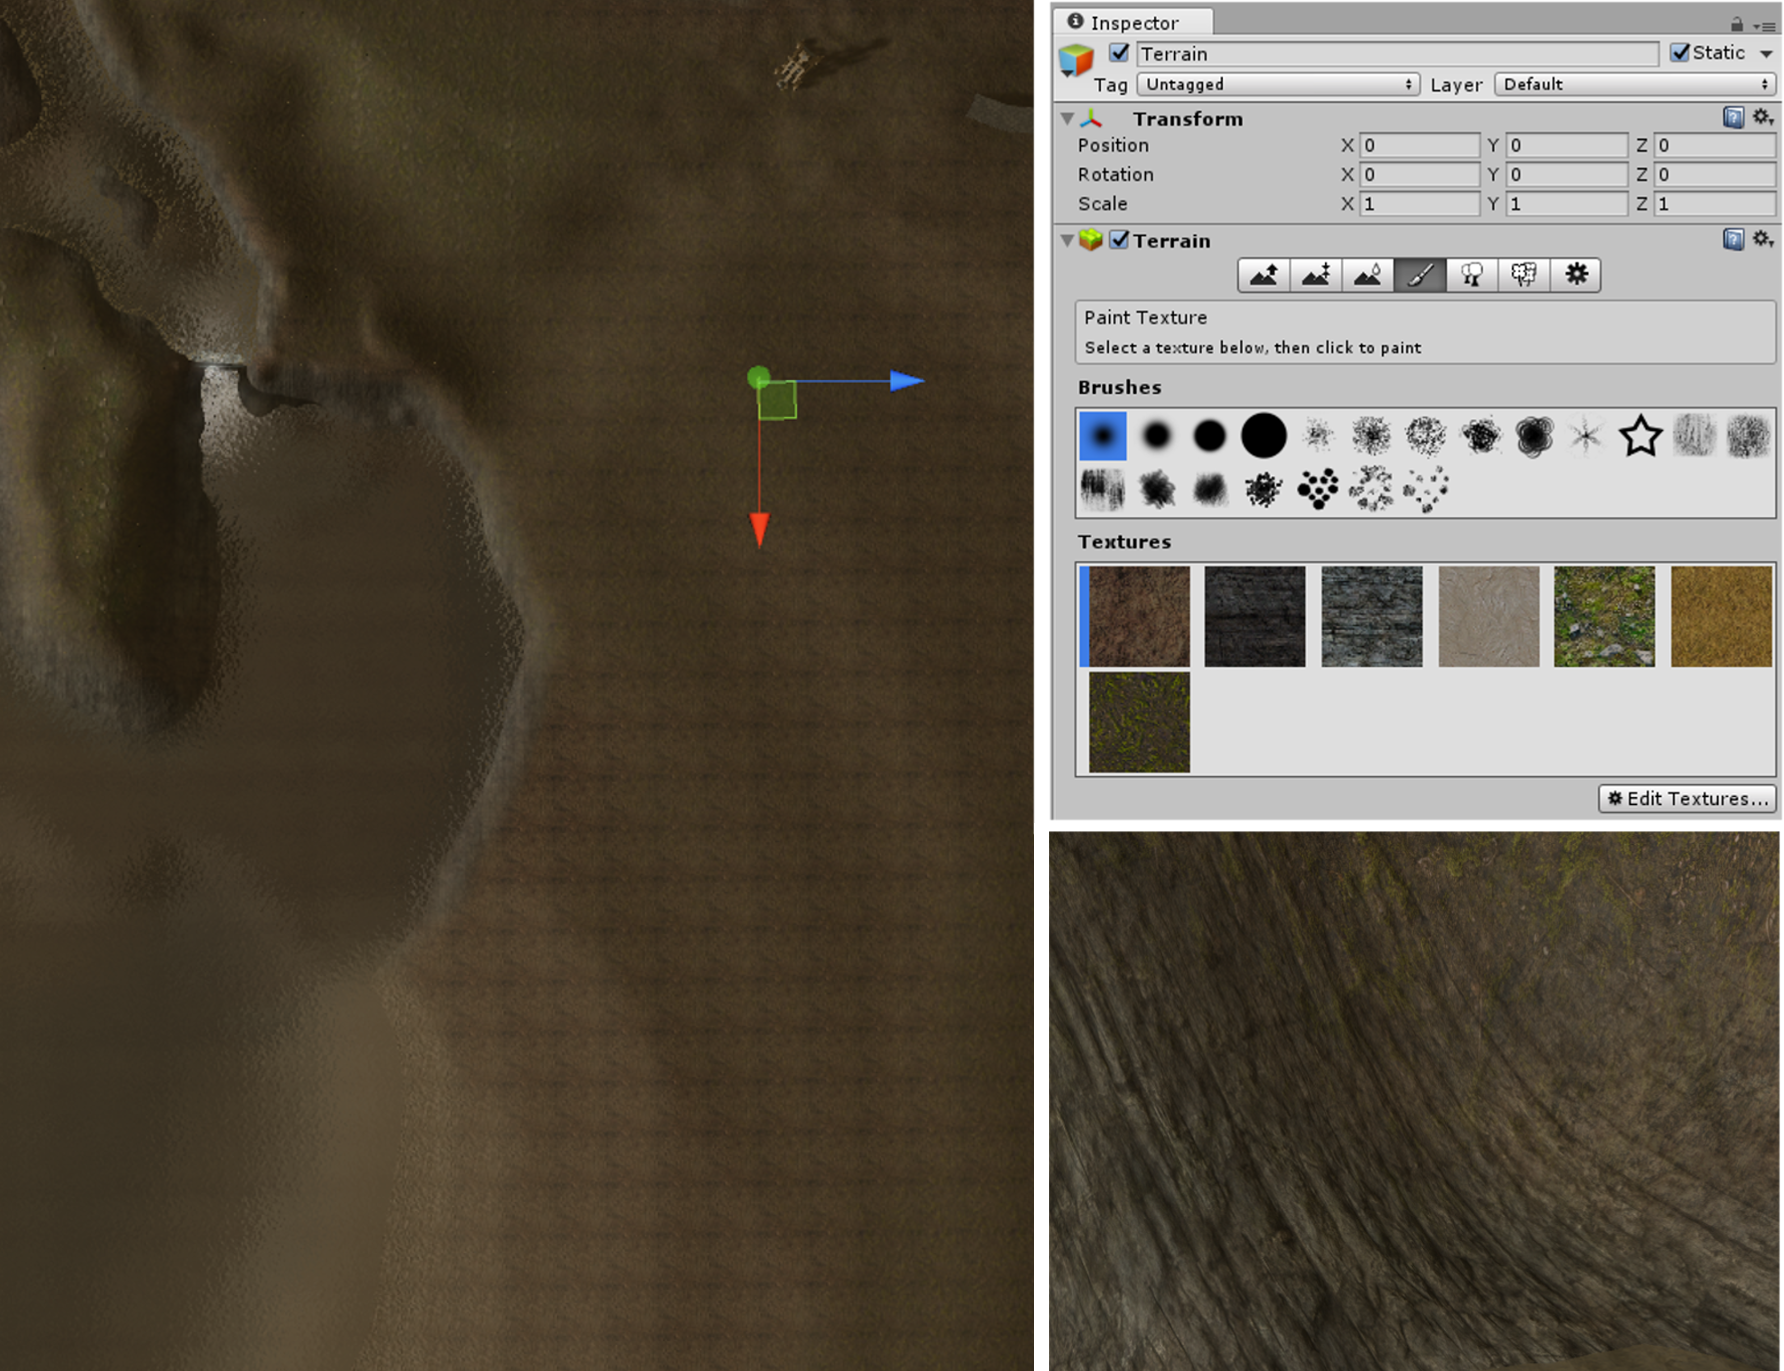
\includegraphics[width=0.95\linewidth]{Abbildungen/Unity/Texture}
	\caption{Wasserebenen und exemplarische Einstellungen}
	\label{fig:Textures}
\end{figure}

Das Gelände mit Texturen zu versehen ist in Unity denkbar einfach und selbsterklärend. Die Abb. \ref{fig:Textures} zeigt das Werkzeug zum Bemalen des Geländes. Es ist vergleichbar mit gängigen Grafikprogrammen. Über die Schaltfläche \textit{Edit Textures} können neue Texturen hinzugefügt werden. Danach stehen diese zur Verfügung und werden mithilfe des Pinsels auf das Gelände aufgetragen. Links in der Abbildung sind die weichen Übergänge von Sand, Erde, Gras und Fels sehen. Diese werden durch geringe Deckkrafteinstellungen und mehrmaliges Auftragen der Texturen erreicht. Eher schroffe Übergänge, unten rechts zu sehen, können durch höhere Deckkraft- und Stärkewerte (\textit{Target Strength}) erzielt werden. Die verwendeten Texturen stammen aus dem Assetstore.

\subsection{Wasser und Wasserfälle}
\subsubsection{Wasser}
In der Szene werden für die Darstellung von Flüssen und Ozean drei Wasserebenen benutzt. Als Asset wird das Standardwasser \textit{WaterProTime} aus Unity verwendet. In Abb. \ref{fig:Water} sind die drei Ebenen (1. kleiner Fluss, 2. großer Fluss und 3. Ozean) zu sehen. Zur Visualisierung des Gefälles wurden die Wasserebenen der Flüsse, im Bild rechts für Ebene 2. zu sehen, geneigt. Schwierigkeiten bei der Verwendung mehrerer Wasserebenen ergeben sich beim Übergang zwischen Zweien und der Wechselwirkung mit dem Gelände. Die Übergänge können beispielsweise durch die Verwendung von Wasserfällen kaschiert werden. 

\begin{figure}[h]
	\centering
	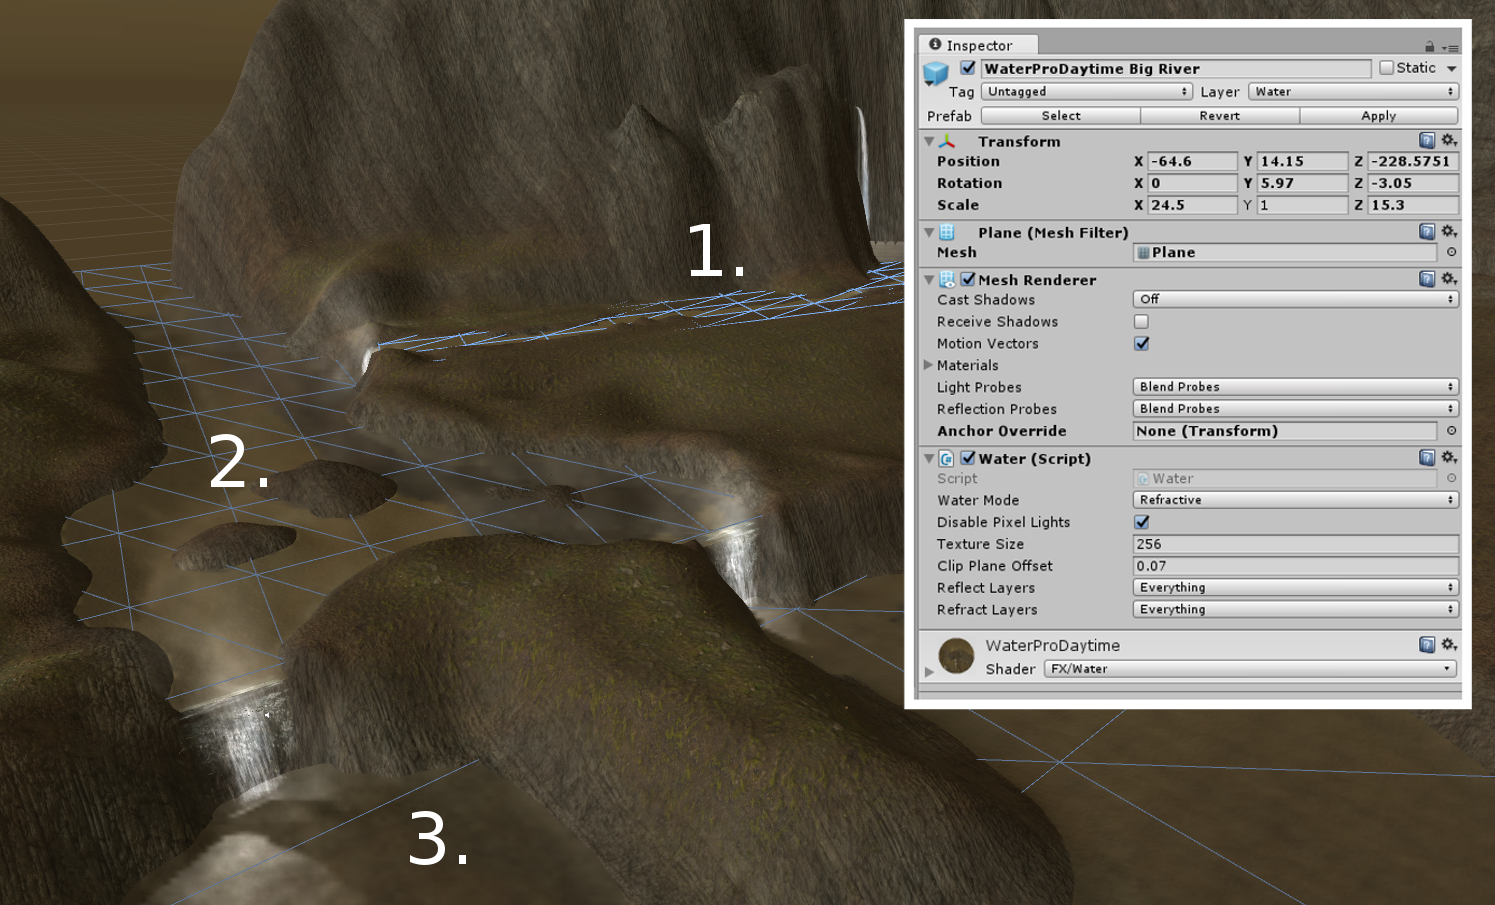
\includegraphics[width=0.95\linewidth]{Abbildungen/Unity/Water}
	\caption{Wasserebenen und exemplarische Einstellungen}
	\label{fig:Water}
\end{figure}

\subsubsection{Wasserfälle}
\begin{wrapfigure}{r}{0.5\textwidth}
	%\vspace{-20pt}
	\begin{center}
		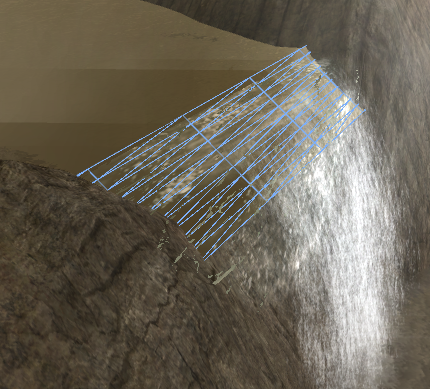
\includegraphics[width=0.45\textwidth]{Abbildungen/Unity/Waterfall}
	\end{center}
	\caption{Wasserfall}
	\label{fig:Waterfall}
\end{wrapfigure}

Trotz der Neigung der Flüsse konnten die Höhenunterschiede zwischen den Wasserebenen nicht ausgeglichen werden. Dadurch wurde es notwendig Wasserfälle in die Szene einzufügen. Diese stammen aus dem Assetstore und wurden für die Zwecke des Projektes angepasst. Die Abb. \ref{fig:Waterfall} zeigt den Übergang zwischen dem kleinen und großen Fluss. Um den harten Wechsel von Wasserebene zu Wasserfall abzuschwächen, war es nötig eine kleine abgeschrägte Ebene passgenau einzufügen. Ebenso mussten die seitlichen Ränder mit dem Terrainwerkzeug verdeckt werden. Diese Technik wurde auch bei den beiden anderen Wasserfällen vom großen Fluss zum Ozean angewendet.

\subsection{Animationen}
\subsubsection{Unity Animationen}
\begin{figure}[h]
	\centering
	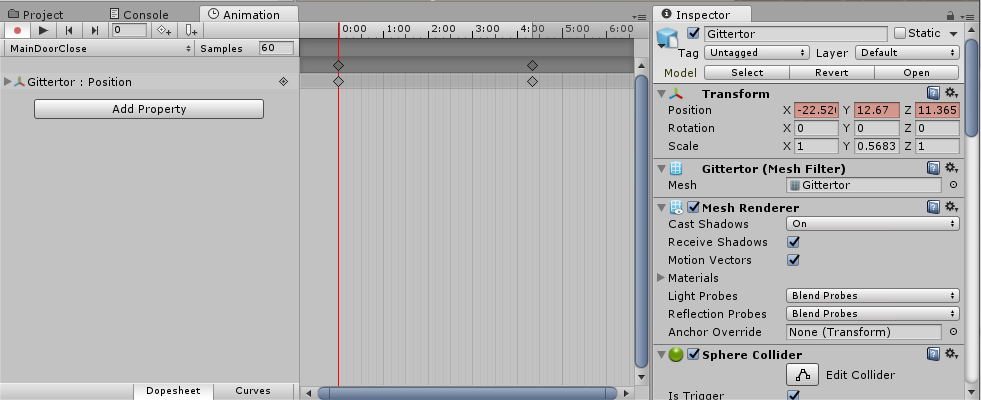
\includegraphics[width=0.95\linewidth]{Abbildungen/Unity/UnityAnim2}
	\caption{Erstellung von Animationen in Unity}
	\label{fig:unityAnim}
\end{figure}

Einfache Animationen, wie das Öffnen eines Burgtores können in Unity schnell und unkompliziert erstellt werden. In Abb. \ref{fig:unityAnim} ist das Werkzeug zur Erstellung von Animationen zu sehen. Im mittleren Teil sieht man die Keyframes und rechts die dazugehörigen \textit{Transform}-Werte. In unserem Fall des Burgtores wird das Schließen über zwei Keyframes mit unterschiedlichen Y-Werten definiert. Die so erstellten Animation stehen später im Animation Controller zur Verfügung.

\subsubsection{3d Studio Max Animation}

\begin{wrapfigure}{r}{0.6\textwidth}
	%\vspace{-20pt}
	\begin{center}
		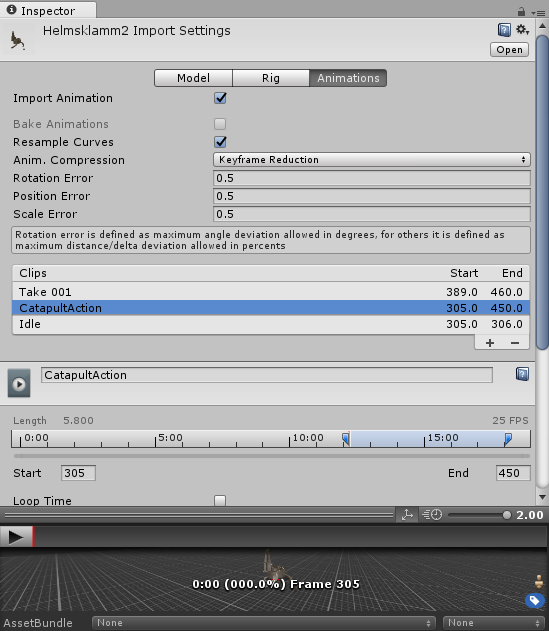
\includegraphics[width=0.55\textwidth]{Abbildungen/Unity/3dsAnim}
	\end{center}
	\caption{Animation aus 3d Studio Max}
	\label{fig:3dsAnim}
\end{wrapfigure}

Kommen die Animationen eines Modells aus 3d Studio Max liegen diese in einer Animationsspur im importierten Asset vor. Durch die Auswahl des Assets in der Assetübersicht können die einzelnen Animationen aus der gemeinsamem Spur extrahiert werden. In Abb. \ref{fig:3dsAnim} ist das benötigte Werkzeug zu sehen. Für unser Hauptmodell sieht man Beispielsweise die Zerstörungsanimation, die in den Keyframes 305 bis 450 vorliegt. Über die Plus-Schaltfläche können auch andere Animationen selektiert werden. Die auf diese Weise extrahierten Einzelanimationen stehen auf die gleiche Art und Weise, wie die in Unity erstellten zur Verfügung.  

\subsubsection{Animation Controller}

Der Animation Controller ist der bevorzugte Weg um Animationen zu kontrollieren und sie abzuspielen. Es handelt sich darin um einen Zustandsautomaten. In jedem Zustand wird eine Animation abgespielt. Übergänge von einem zum anderen bewirkt das Abspielen einer neuen Bewegung. Die Übergänge zwischen zwei Zuständen können mit Bedingungen versehen werden. In Abb. \ref{fig:animController} sieht man den Controller für das Burgtor. Zu Beginn der Szene wird in den \textit{MainDoorClosed} Zustand gewechselt. In diesem wird eine Ruhe-Animation abgespielt, welche dem geschlossenen Tor entspricht. Per Skript kann die Variable \textit{open} gesetzt werden und es erfolgt der Wechsel in den Zustand \textit{MainDoorOpen} der die Animation zum Öffnen des Tores abspielt. Ist diese beendet, wechselt der Automat in den Ruhe-Zustand des geöffneten Burgtores. Von diesem Zustand aus, kann über das Setzen der Variable \textit{close}, zum geschlossenen gewechselt werden. Über den Controller können auch Überblendungen zwischen den Animationen eingestellt werden. Die Einstellung dafür sind auf der rechten Seite der Abbildung zu sehen. So wird es möglich auch zwei Animationen nahtlos ineinander übergehen zu lassen. 


\begin{figure}[h]
	\centering
	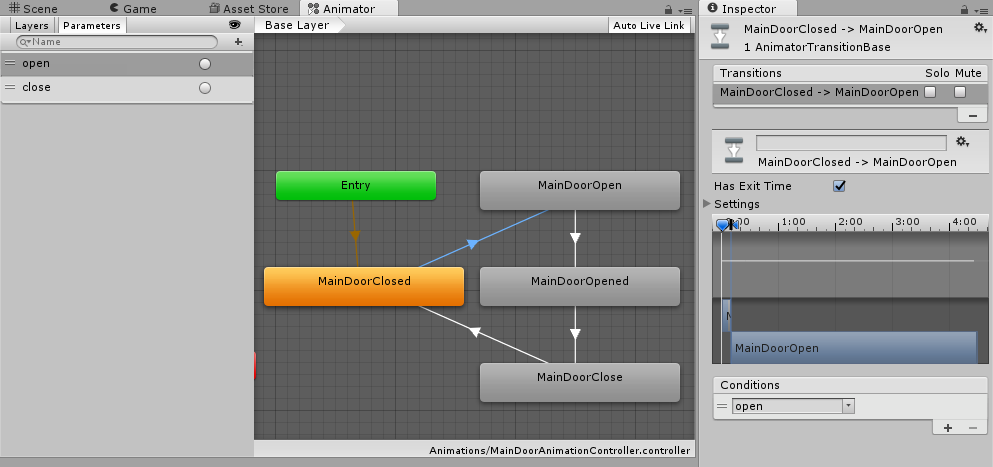
\includegraphics[width=0.95\linewidth]{Abbildungen/Unity/AnimationController}
	\caption{Animation-Controller zur Steuerung von Animationen}
	\label{fig:animController}
\end{figure}

\newpage
\subsection{Partikelsystem Fackel}
In wenigen Schritten und mithilfe des Partikelsystems in Unity kann man in kürzester Zeit schöne Feuereffekte erstellen.

\begin{figure}[H]
\centering
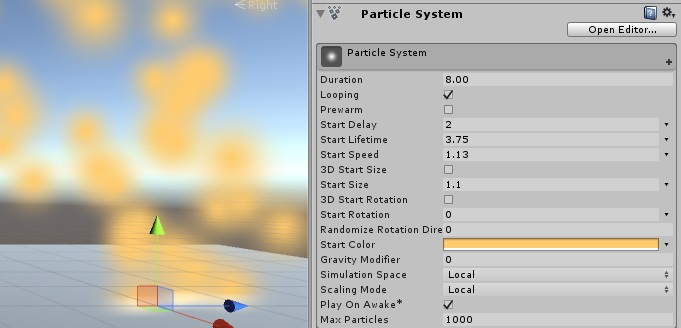
\includegraphics[width=0.95\linewidth]{Abbildungen/Unity/Fire/fire1}
\caption{Grundeinstellung Partikelsystem}
\label{fig:fire1}
\end{figure}

Im ersten Schritt wird ein Gameobject \textit{Particle System} erstellt und die in Abb. \ref{fig:fire1} abgebildeten Grundeinstellungen vorgenommen.

\begin{figure}[h!]
\centering
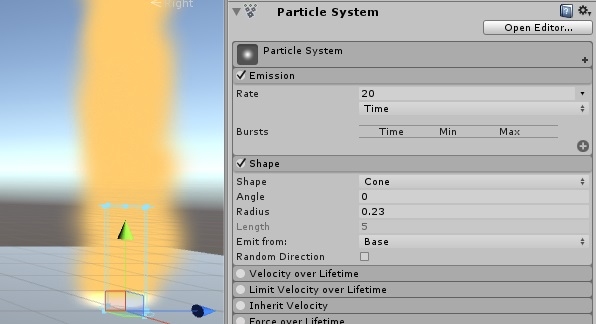
\includegraphics[width=0.95\linewidth]{Abbildungen/Unity/Fire/fire2}
\caption{Einstellungen Emission und Shape}
\label{fig:fire2}
\end{figure}

Um die Partikel zu verdichten und die horizontale Streuung einzugrenzen, wird die Emission erhöht und die Form angepasst. (siehe Abb.\ref{fig:fire2}) 

\begin{figure}[h!]
\centering
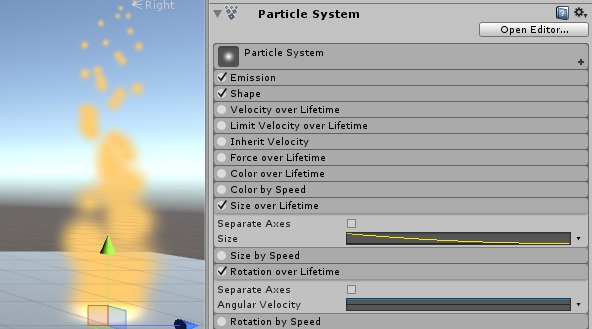
\includegraphics[width=0.95\linewidth]{Abbildungen/Unity/Fire/fire3}
\caption{Einstellungen \textit{Size over Livetime} und \textit{Rotation over Lifetime}}
\label{fig:fire3}
\end{figure}

Die typische Flammenform erreicht man, indem man die Größe im Bezug zur Lebensdauer anpasst. Dazu wählt man eine exponentiell sinkende Kurve. Außerdem versetzt man die Partikel in eine Rotation. (siehe Abb. \ref{fig:fire3})

\begin{figure}[h!]
\centering
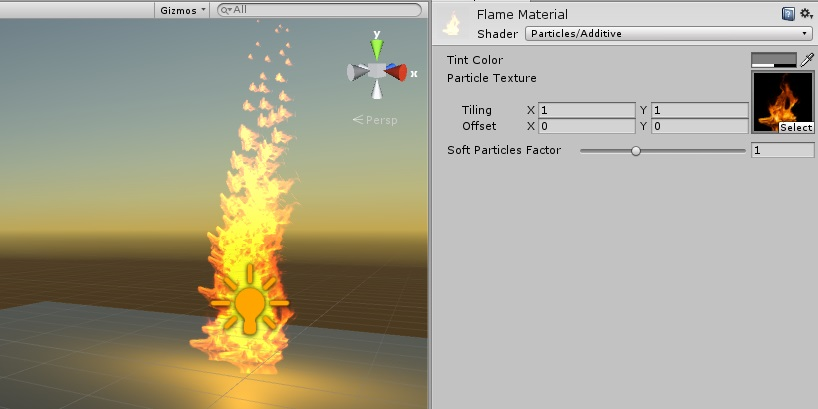
\includegraphics[width=0.95\linewidth]{Abbildungen/Unity/Fire/fire4}
\caption{Material und Point Light}
\label{fig:fire4}
\end{figure}

Um einen Flammenähnlichen Farbverlauf zu erreichen, muss man dem Partikelsystem ein Material zufügen. Dieses besteht aus dem Bild einer Flame auf schwarzem Hintergrund und entfaltet durch den Shader \textit{Particles/Additive} den gewünschten Effekt.

\newpage

\subsection{Benutzeroberfläche}

\begin{figure}[h]
	\centering
	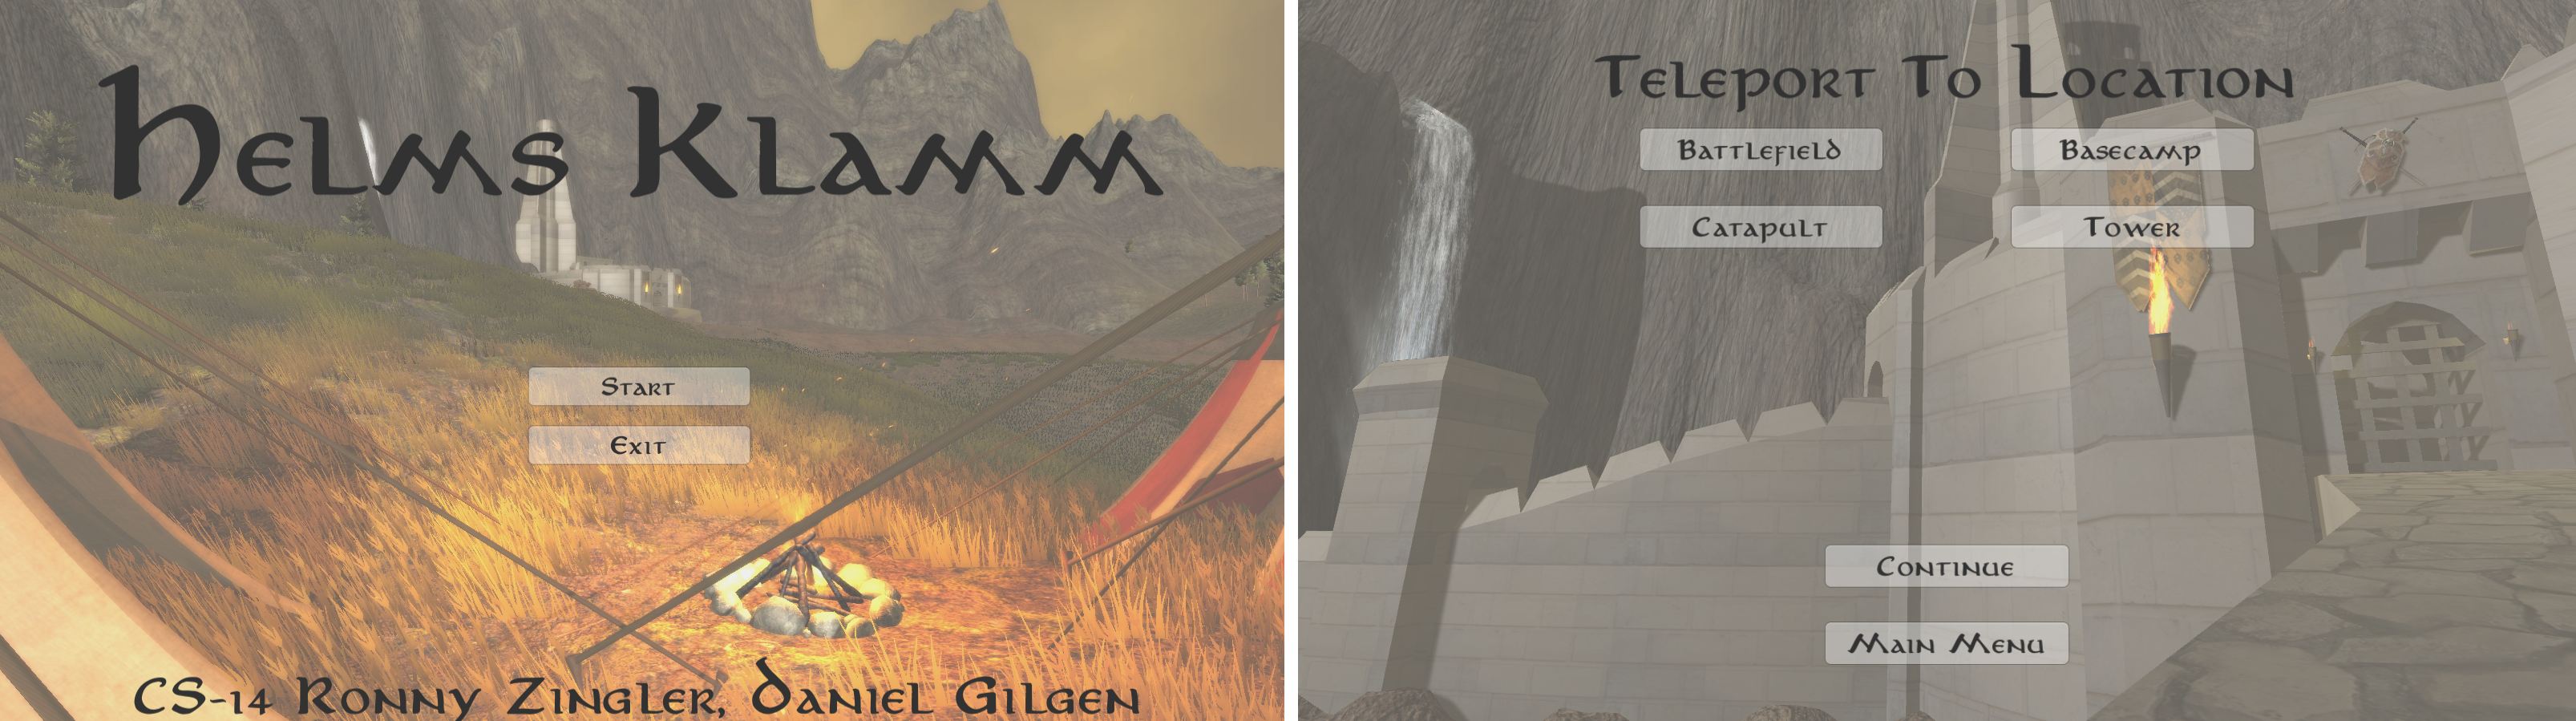
\includegraphics[width=0.95\linewidth]{Abbildungen/Unity/GuiCombined}
	\caption{Graphische Nutzeroberflächen}
	\label{fig:GuiCombined}
\end{figure}

%\begin{figure}[h]
%	\centering
%	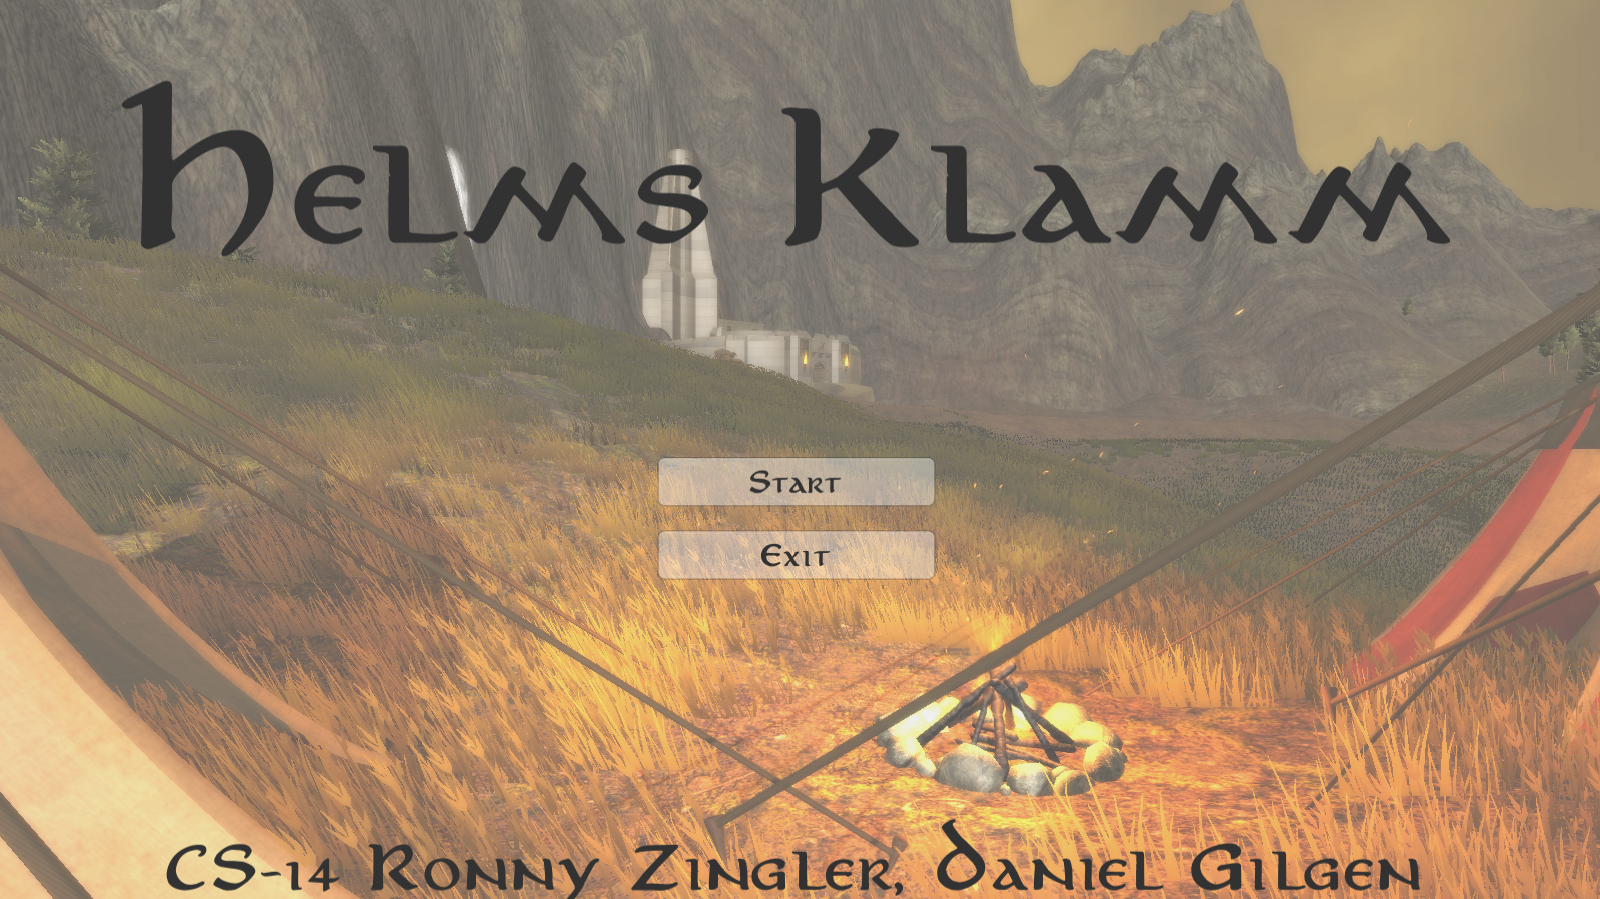
\includegraphics[width=0.95\linewidth]{Abbildungen/Unity/MainMenu}
%	\caption{Hauptmenü}
%	\label{fig:mainMenu}
%\end{figure}
%
%\begin{figure}[H]
%	\centering
%	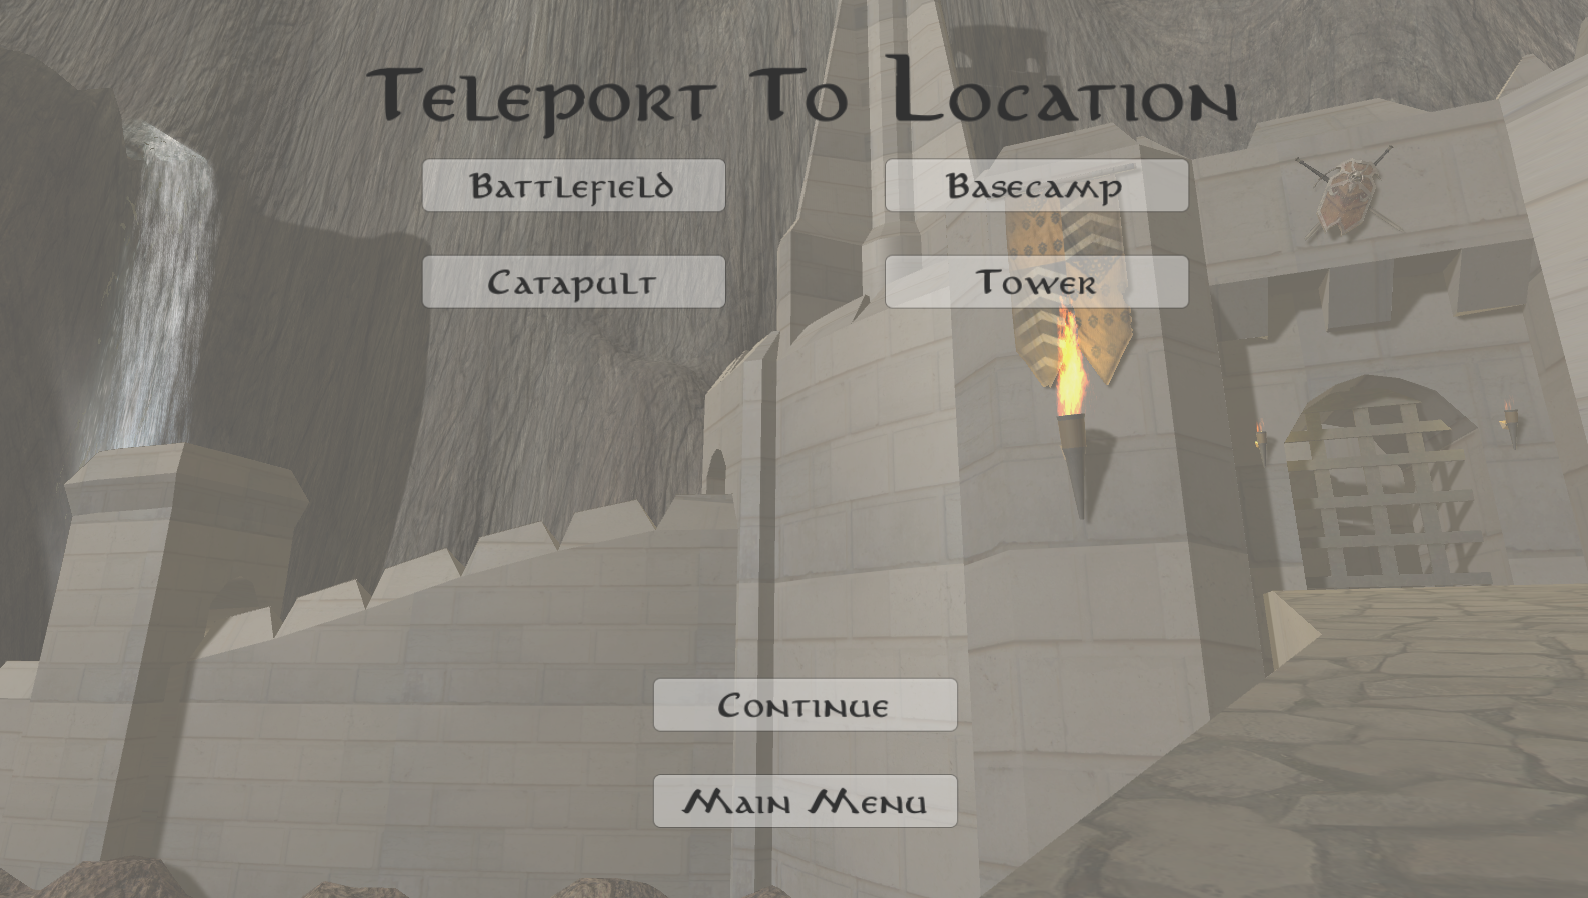
\includegraphics[width=0.95\linewidth]{Abbildungen/Unity/IngameMenu}
%	\caption{Spielmenü}
%	\label{fig:ingameMenü}
%\end{figure}

%\begin{wrapfigure}{r}{0.6\textwidth}
%
%	\begin{center}
%		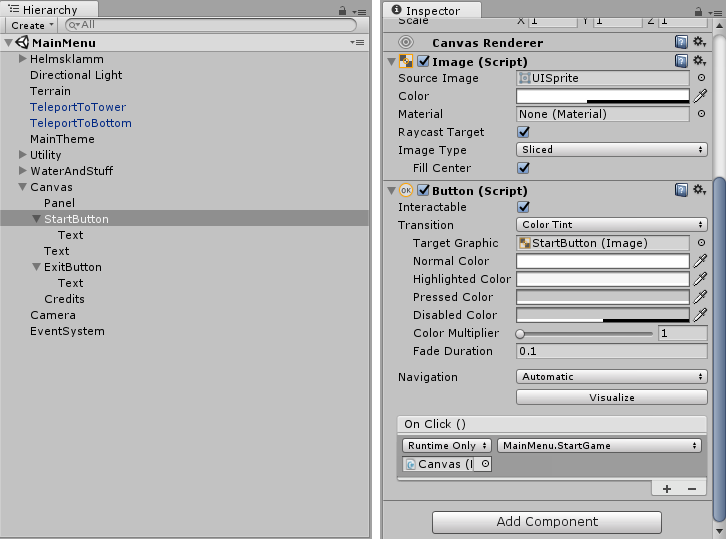
\includegraphics[width=0.55\textwidth]{Abbildungen/Unity/GuiExample}
%	\end{center}
%	\caption{Hierarchie und Inspektor für Startbutton}
%	\label{fig:3dsAnim}
%\end{wrapfigure}

\begin{figure}[h]
	\centering
	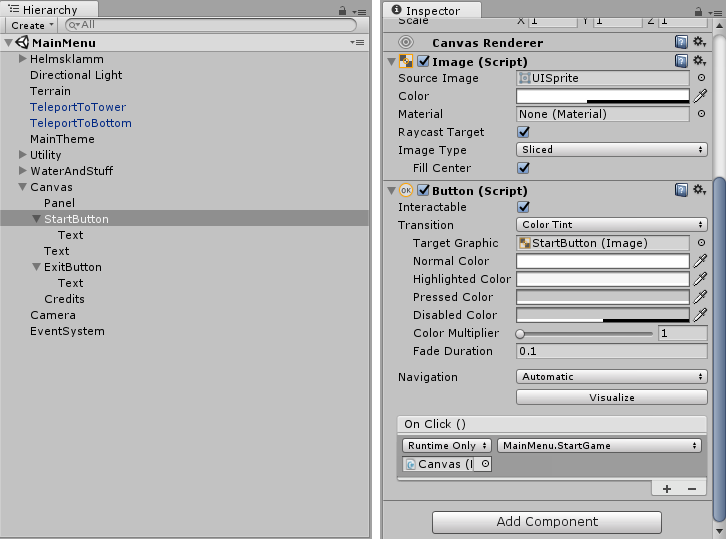
\includegraphics[width=0.95\linewidth]{Abbildungen/Unity/GuiExample}
	\caption{Hierarchie und Inspektor für Startbutton}
	\label{fig:GuiExample}
\end{figure}

Zur Erstellung von graphischen Nutzeroberflächen stehen in Unity vergleichbare Elemente wie in gängigen Programmiersprachen zur Verfügung. Grundelement einer jeden Benutzeroberfläche sind die \textit{Canvas}. In diese werden die Elemente über den Editor eingefügt, positioniert und individualisiert.  Es gibt verschiedene Möglichkeiten zur Darstellung. Für diesen Anwendungsfall wurde die Darstellungsart \textit{Screen Space - Overlay} gewählt. Dadurch werden die Elemente der Benutzeroberfläche bildschirmfüllend über die Szene gelegt. In Abbildung \ref{fig:GuiCombined} sieht man links das Haupt- und rechts das Spielmenü. Der generelle Aufbau beider Oberflächen ist sehr ähnlich. In Abb. \ref{fig:GuiExample} ist der Szenengraph des Hauptmenüs und die exemplarischen Einstellungen des Start-Buttons zu sehen. Die Szene des Hauptmenüs wurde von der eigentlichen abgeleitet. Unterschied ist die feste Kamera anstatt des \textit{FPS-Controllers} und die Entfernung jeglicher Umgebungsgeräusche. Stattdessen wird während der Darstellung des Hauptmenüs eine eingängige Musik abgespielt. Unten rechts in Abb. \ref{fig:GuiExample} ist zu sehen was beim Klicken des Start-Button erfolgt. In unserem Fall wird dadurch in die eigentliche Spielszene gewechselt.

\subsection{Audio}

\begin{wrapfigure}{r}{0.5\textwidth}
	\vspace{-20pt}
	\begin{center}
		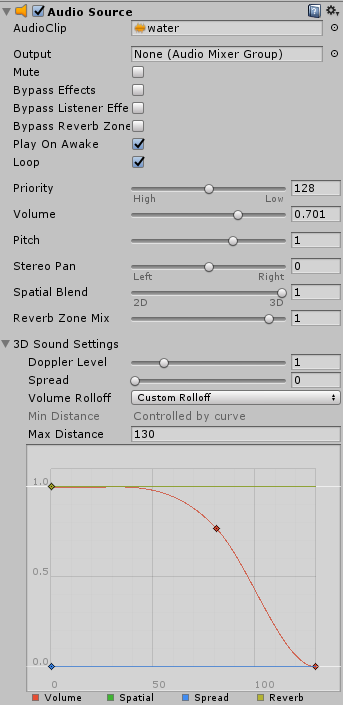
\includegraphics[width=0.45\textwidth]{Abbildungen/Unity/calmWaterAudio}
	\end{center}
	\caption{Audioeinstellungen}
	\label{fig:audioExample}
\end{wrapfigure}

Audioquellen können auf die gleiche Art und Weise wie 3d Objekte in der Welt platziert werden. Um diese zu hören, muss auf einem anderen Objekt ein \textit{Audio Listener} vorhanden sein. Im Fall unseres Projektes macht es nur Sinn, diesen bei einer Kamera oder dem Charakter zu platzieren. Das Platzieren zweier \textit{Listener} zur gleichen Zeit muss unbedingt vermieden werden. Abb. \ref{fig:audioExample} zeigt die Einstellungen der Wasserhintergrundgeräusche. Im oberen Teil ist sichtbar, dass die Geräusche sofort zum Beginn der Szene abgespielt werden und danach, bis zum Schließen dieser, wiederholt wird. Es ist natürlich ebenso möglich, Musik oder Tonquellen programmatisch zu starten. Im unteren Teil sind die Einstellungen zum Zusammenhang zwischen Entfernung und Lautstärke zu sehen. Im Falle des Wassergeräusches wurde eine eigene Kurve gewählt. Der Grund für diese Entscheidung, war das Vorhandensein zwei Tonquellen mit dem gleichen Geräusch. Nur dadurch war ein zufriedenstellendes Ergebnis für das plätschernde Geräusch des Wassers zu erreichen. Normalerweise genügen aber die beiden vordefinierten Lautstärke Kurven, logarithmisch und linear. Damit die \textit{3D Sound Settings} wirken, darf der Regler \textit{Spatial Blend} nicht auf 2D eingestellt werden.




 

